%%%%%%%%%%%%%%%%%%%%%%%%%%%%%%%%%%%%%
%                                   %
% Compile with XeLaTeX and biber    %
%                                   %
% Questions or comments:            %
%                                   %
% joshua dot mcneill at uga dot edu %
%                                   %
%%%%%%%%%%%%%%%%%%%%%%%%%%%%%%%%%%%%%

\documentclass{beamer}
  % Read in standard preamble (cosmetic stuff)
  %%%%%%%%%%%%%%%%%%%%%%%%%%%%%%%%%%%%%%%%%%%%%%%%%%%%%%%%%%%%%%%%
% This is a standard preamble used in for all slide documents. %
% It basically contains cosmetic settings.                     %
%                                                              %
% Joshua McNeill                                               %
% joshua dot mcneill at uga dot edu                            %
%%%%%%%%%%%%%%%%%%%%%%%%%%%%%%%%%%%%%%%%%%%%%%%%%%%%%%%%%%%%%%%%

% Beamer settings
% \usetheme{Berkeley}
\usetheme{CambridgeUS}
% \usecolortheme{dove}
% \usecolortheme{rose}
\usecolortheme{seagull}
\usefonttheme{professionalfonts}
\usefonttheme{serif}
\setbeamertemplate{bibliography item}{}

% Packages and settings
\usepackage{fontspec}
  \setmainfont{Charis SIL}
\usepackage{hyperref}
  \hypersetup{colorlinks=true,
              allcolors=blue}
\usepackage{graphicx}
  \graphicspath{{../../figures/}}
\usepackage[normalem]{ulem}
\usepackage{enumerate}

% Document information
\author{M. McNeill}
\title[FREN2001]{Français 2001}
\institute{\url{joshua.mcneill@uga.edu}}
\date{}

%% Custom commands
% Lexical items
\newcommand{\lexi}[1]{\textit{#1}}
% Gloss
\newcommand{\gloss}[1]{`#1'}
\newcommand{\tinygloss}[1]{{\tiny`#1'}}
% Orthographic representations
\newcommand{\orth}[1]{$\langle$#1$\rangle$}
% Utterances (pragmatics)
\newcommand{\uttr}[1]{`#1'}
% Sentences (pragmatics)
\newcommand{\sent}[1]{\textit{#1}}
% Base dir for definitions
\newcommand{\defs}{../definitions}


  % Packages and settings
  \usepackage[style=apa, backend=biber]{biblatex}
    \addbibresource{../references/References.bib}

  % Document information
  \subtitle[Variation and Varieties]{Introduction to Language Variation and Language Varieties}

  %% Custom commands
  % Subsection/frame titles
  \newcommand{\suboneone}{What are we looking at?}
  \newcommand{\subtwoone}{What do we mean by ``variety''?}
  \newcommand{\subtwotwo}{Dialects}
  \newcommand{\subtwothree}{Other lects and registers}
  \newcommand{\subtwofour}{Idiolects and styles}
  \newcommand{\subtwofive}{Jargon and slang}
  \newcommand{\subtwosix}{Standards}
  \newcommand{\subtwoseven}{Practice}

\begin{document}
  % Read in the standard intro slides (title page and table of contents)
  %%%%%%%%%%%%%%%%%%%%%%%%%%%%%%%%%%%%%%%%%%%%%%%%%%%%%%%%%%%%%%%%
% This is a standard set of intro slides used in for all slide %
% documents. It basically contains the title page and table of %
% contents.                                                    %
%                                                              %
% Joshua McNeill                                               %
% joshua dot mcneill at uga dot edu                            %
%%%%%%%%%%%%%%%%%%%%%%%%%%%%%%%%%%%%%%%%%%%%%%%%%%%%%%%%%%%%%%%%

\begin{frame}
  \titlepage
  \tiny{Office: % Basically a variable for office hours location
Gilbert 121\\
        Office hours: % Basically a variable for office hours
 lundi, mercredi, vendredi 10:10--11:10
}
\end{frame}

\begin{frame}
  \tableofcontents[hideallsubsections]
\end{frame}

\AtBeginSection[]{
  \begin{frame}
    \tableofcontents[currentsection,
                     hideallsubsections]
  \end{frame}
}


  \section{Intro to Variation}
    \subsection{\suboneone}
      \begin{frame}{\suboneone}
        \begin{block}{Are there differences between these?}
          \begin{tabular}{r l @{ vs } l}
            1)  & English                                       & Japanese                            \\
            2)  & English in the UK                             & English in the US                   \\
            3)  & English in Georgia                            & English in New Jersey               \\
            4)  & English in Athens                             & English in rural Georgia            \\
            5)  & \multicolumn{2}{l}{English of different communities in Athens}                      \\
            6)  & \multicolumn{2}{l}{English of different individuals within one} \\
                & \multicolumn{2}{l}{community in Athens} \\
            7)  & \multicolumn{2}{l}{Your English in different contexts}
          \end{tabular}
        \end{block}
      \end{frame}

      \begin{frame}{\suboneone}
        \begin{alertblock}{Language variation}
          % Language variation
That part of sociolinguistics that deals with how language varies between communities, between individuals, and within individuals

        \end{alertblock}
        \begin{alertblock}{Sociolinguistics}
          % Sociolinguistics
The study of how language interacts with society and culture

        \end{alertblock}
      \end{frame}

  \section{Language Varieties}
    \subsection{\subtwoone}
      \begin{frame}{\subtwoone}
        \begin{alertblock}{Variety}
          % Variety
Any systematic or systematic-like form of language

        \end{alertblock}
        \begin{block}{Types of varieties}
          Socio-political varieties (i.e., systematic-like)
          \parbox{0.48\linewidth}{
            \begin{itemize}
              \item Languages
              \item Dialects
              \item Sociolects
            \end{itemize}
          }
          \parbox{0.48\linewidth}{
            \begin{itemize}
              \item Ethnolects
              \item Registers
              \item[]
            \end{itemize}
          }
          Real systems
          \begin{itemize}
            \item Idiolects
            \item Styles
          \end{itemize}
        \end{block}
      \end{frame}

      \begin{frame}{\subtwoone}
        \begin{block}{Dimensions of variation}
          \begin{itemize}
            \item Lexical variation
            \item Grammatical variation
            \begin{itemize}
              \item i.e., Syntax, morphology, phonology
              \item \alert{Accent}: % Accent
The phonology associated with a variety

            \end{itemize}
          \end{itemize}
        \end{block}
      \end{frame}

    \subsection{\subtwotwo}
      \begin{frame}[t]{\subtwotwo}
        \begin{definition}
          % Dialect
A geographically defined variety

        \end{definition}
        \only<1>{
          \begin{columns}
            \column{0.5\linewidth}
            \begin{alertblock}{}
              This is not a disparaging term in linguistics
            \end{alertblock}
            \begin{example}
              Appalachian English vs New York English
            \end{example}
            \column{0.5\linewidth}
            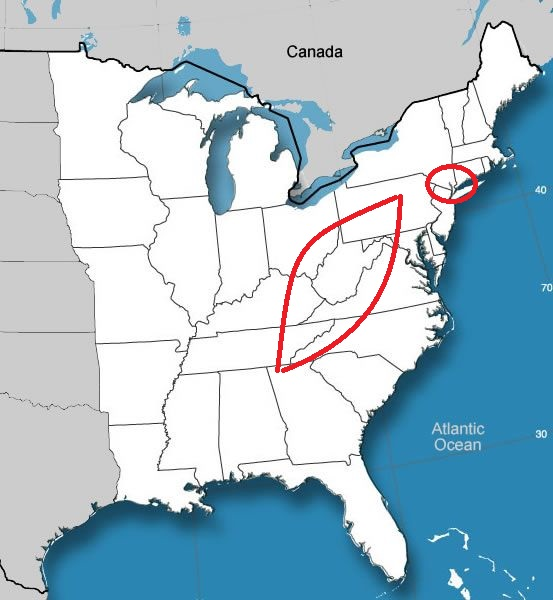
\includegraphics[scale=0.25]{appalachia_new_york.jpg}
          \end{columns}
        }
        \only<2-4>{
          \begin{columns}
            \column{0.5\linewidth}
              \begin{minipage}[t][0.6\textheight]{\linewidth}
                \only<2>{
                  \begin{alertblock}{Speech community}
                    % Speech community
A geographically defined community that shares ways of speaking as well as evaluations for those ways of speaking
 \parencite{labov_social_2006}
                  \end{alertblock}
                }
                \only<3>{
                  \begin{block}{Extra-linguistic factors that divide up speech communities}
                    \begin{itemize}
                      \item Socioeconomic status
                      \item Age
                      \item Gender
                      \item Ethnicity
                    \end{itemize}
                  \end{block}
                }
                \only<4>{
                  \begin{block}{Not the only conceptualization of community}
                    Speech communities work well for large demographically-driven surveys
                  \end{block}
                }
              \end{minipage}
            \column{0.5\linewidth}
              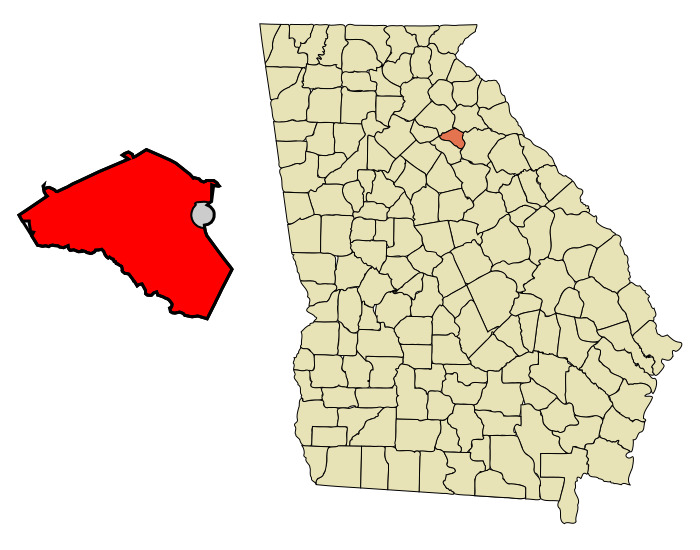
\includegraphics[scale=0.2]{athens.jpg}
          \end{columns}
        }
      \end{frame}
      \begin{frame}[t]{\subtwotwo}
        \begin{block}{}
          How do we tell the difference between dialects and languages?
        \end{block}
        \only<2-5>{
          \begin{columns}
            \column{0.5\linewidth}
              \begin{minipage}[t][0.6\textheight]{\linewidth}
                \begin{block}{Mutual intelligibility?}
                  \only<-4>{
                    \begin{itemize}
                      \item \href{https://www.greenvilleonline.com/videos/news/2019/02/04/gullah-dialect-still-spoken-south-carolina/2653241002/}{Difficult to measure}
                      \item<3-> Swedes and Norwegians often understand each other
                      \item<4-> Speakers of different Chinese ``dialects'' often \emph{don't} understand each other
                    \end{itemize}
                  }
                  \only<5->{
                    Also, \alert{dialect continuums}:
                    \begin{itemize}
                      \item % Dialect continuum
A situation in which a number of geographically contiguous dialects exist where each is mutually intelligible with the next but those at either end are not

                    \end{itemize}
                  }
                \end{block}
              \end{minipage}
            \column{0.5\linewidth}
              \only<3>{
                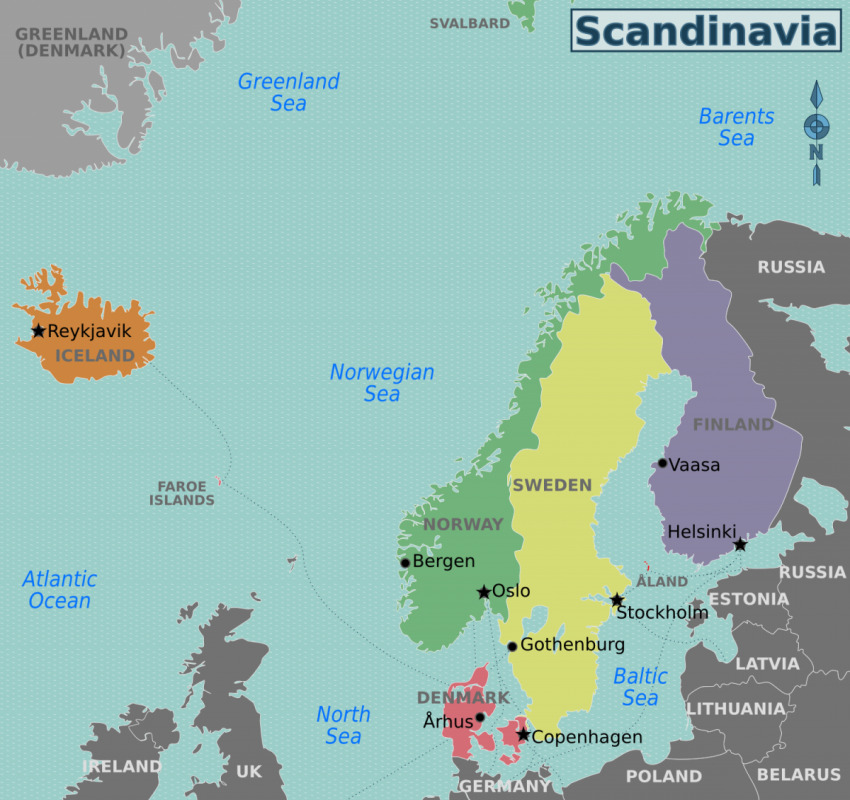
\includegraphics[scale=0.15]{sweden_norway.jpg}
              }
              \only<4>{
                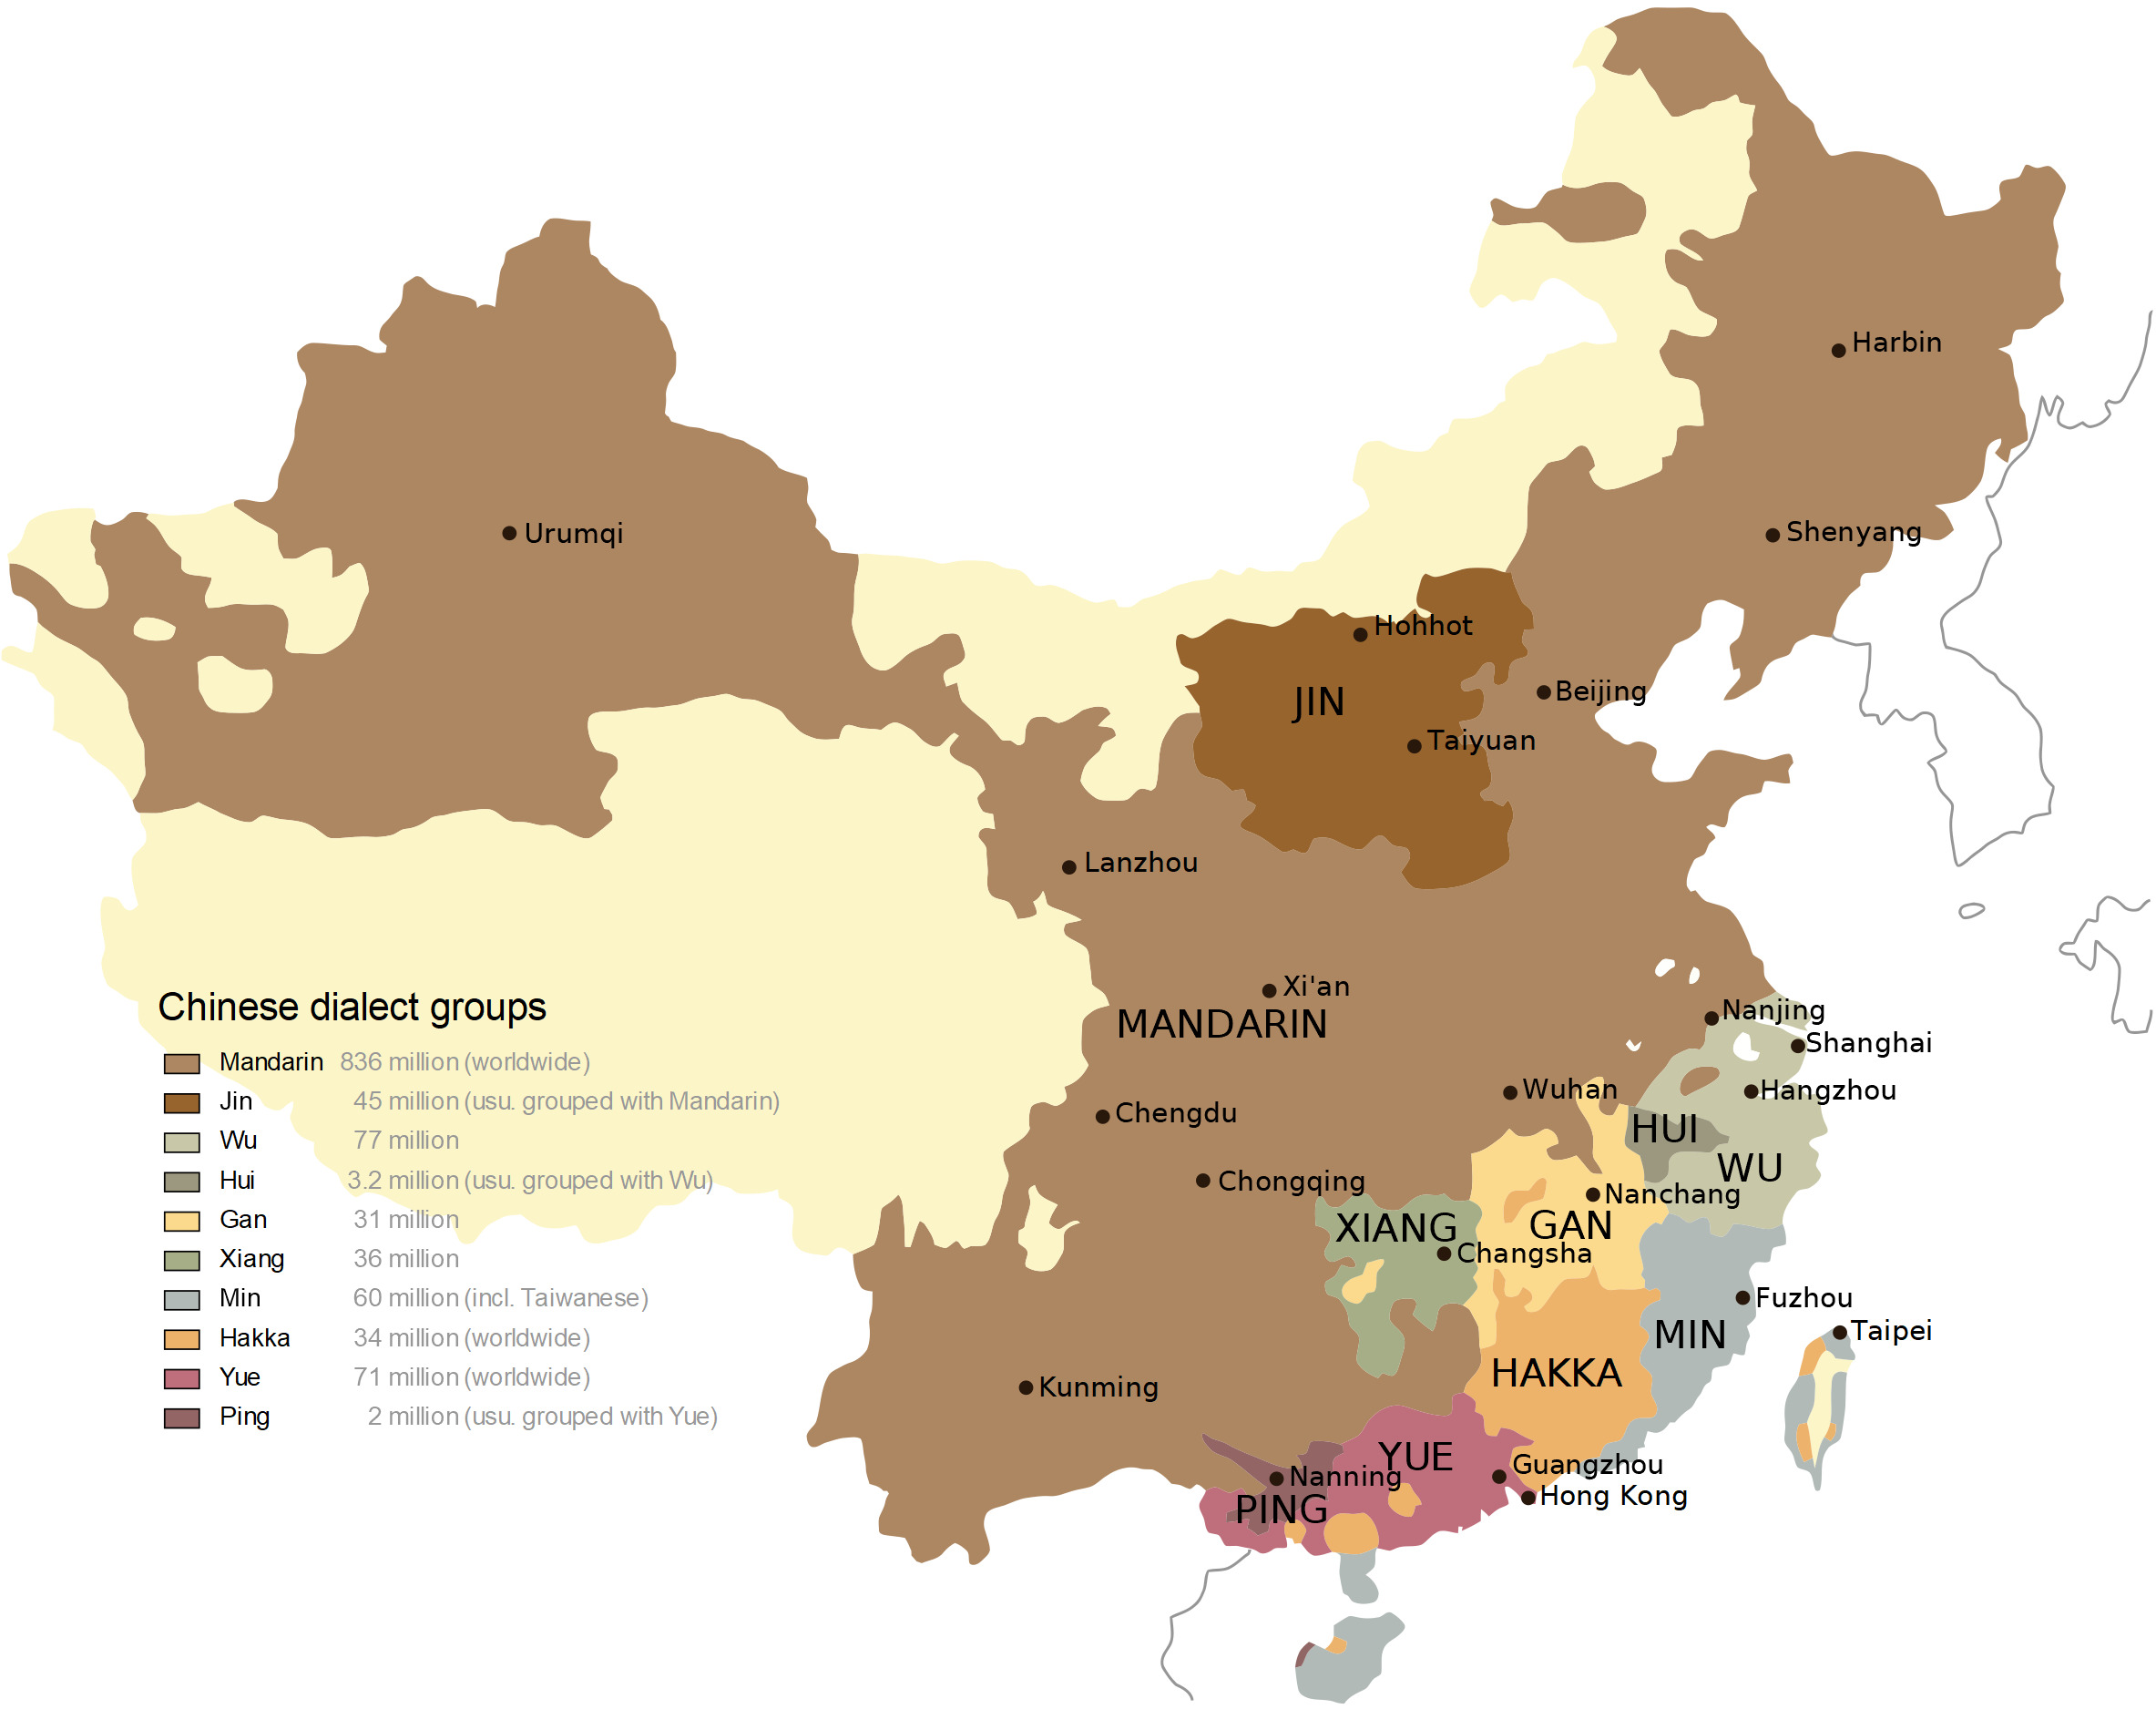
\includegraphics[scale=0.06]{chinese_dialects.jpg}
              }
              \only<5>{
                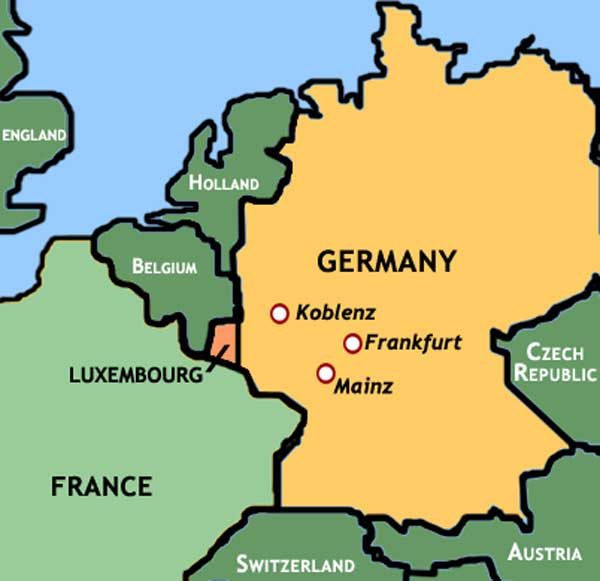
\includegraphics[scale=0.2]{germany_netherlands.jpg}
              }
          \end{columns}
        }
        \only<6>{
          \begin{block}{People decide}
            Languages and dialects are social constructs
          \end{block}
        }
      \end{frame}

    \subsection{\subtwothree}
      \begin{frame}{\subtwothree}
        \begin{alertblock}{Sociolect}
          % Sociolect
A variety defined by social class

          \begin{itemize}
            \item Working-class English vs Upper-class English
          \end{itemize}
        \end{alertblock}
        \begin{alertblock}{Ethnolect}
          % Ethnolect
A variety defined by ethnicity

          \begin{itemize}
            \item African-American English vs Chicano English
          \end{itemize}
        \end{alertblock}
        \begin{alertblock}{Register}
          % Register
A variety defined by activity

          \begin{itemize}
            \item Newscaster speech vs Infant directed speech
          \end{itemize}
        \end{alertblock}
      \end{frame}

    \subsection{\subtwofour}
      \begin{frame}{\subtwofour}
        \begin{block}{How would you greet the Queen of England?}
          \begin{enumerate}
            \item \uttr{Hey, how's it goin'?}
            \item \uttr{It's an honor to meet you, Your Majesty.}
          \end{enumerate}
        \end{block}
      \end{frame}

      \begin{frame}[t]{\subtwofour}
        \begin{alertblock}{Style}
          % Style
A single individual's systematic speech patterns in some context

        \end{alertblock}
        \only<2-3>{
          \begin{alertblock}{Idiolect}
            % Idiolect
A single individual's total repertoire of styles

          \end{alertblock}
          \begin{block}{What does ``context'' mean?}
            \uncover<3->{
            Like in pragmatics:
            \begin{itemize}
              \item Situational context
              \item Social context
            \end{itemize}
            }
          \end{block}
        }
        \only<4->{
          \begin{columns}
            \column{0.5\linewidth}
              \begin{alertblock}{Style shifting}
                % Style shifting
The process of modulating the language style a speaker is using

                \begin{itemize}
                  \item Often, this is subconscious
                  \item Chart from \textcite{labov_social_2006}
                \end{itemize}
              \end{alertblock}
            \column{0.5\linewidth}
              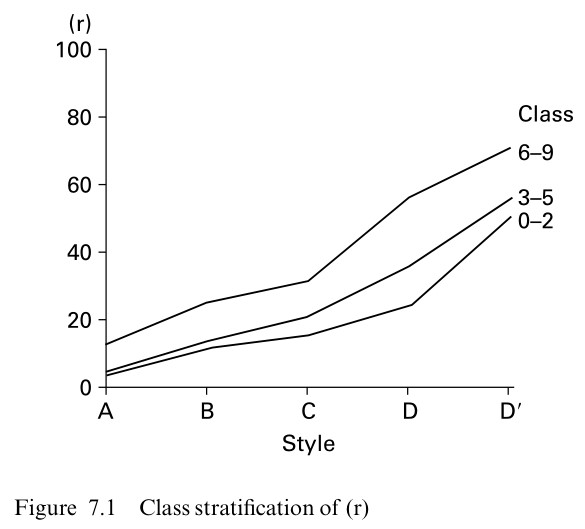
\includegraphics[scale=0.45]{r_stratification.jpg}
          \end{columns}
        }
      \end{frame}

    \subsection{\subtwofive}
      \begin{frame}{\subtwofive}
        \begin{block}{Lexical variation}
          \begin{itemize}
            \item \alert{Jargon}: % Jargon
A set of lexical expressions that are highly specialized for a certain field and unlikely to be understood by those unacquainted with that field

            \item \alert{Slang}: % Slang
A set of (often transitory) lexical expressions that are highly specialized for a certain tight-knit group of people

          \end{itemize}
        \end{block}
        \begin{block}{What are these useful for?}
          \uncover<2->{
            Both express the idea that you're in-the-know
          }
        \end{block}
      \end{frame}

    \subsection{\subtwosix}
      \begin{frame}{\subtwosix}
        \begin{alertblock}{Standard variety}
          % Standard variety
A variety that is considered prestigious typically due to its use by those with power and in educational contexts

          \begin{itemize}
            \item ``Standard'' does \emph{not} mean ``superior''
          \end{itemize}
        \end{alertblock}
        \begin{example}
          Negative concord (i.e., double negation) is non-standard but was standard (Chaucer, 1400):
          \begin{enumerate}
            \item
            \parbox[t]{\linewidth}{
              \begin{tabular}{l l l l l l l}
                He & nevere & yet & no & vileynye & ne  & sayde \\
                He & never  & yet & no & villainy & not & said
              \end{tabular}
              \begin{tabular}{l l l l l l l l}
                In & al  & his & lyf  & unto & no & maner   & wight \\
                In & all & his & life & to   & no & kind of & creature
              \end{tabular}
            }
          \end{enumerate}
        \end{example}
      \end{frame}

      \begin{frame}[t]{\subtwosix}
        \begin{alertblock}{Hypercorrection}
          % Hypercorrection
When a speaker mistakenly uses a prestige form from a standard variety in a linguistic context where it is not supposed to be used

        \end{alertblock}
        \only<-2>{
          \begin{example}
            \begin{enumerate}
              \item \only<2->{\alert{*}}Kim and me went to the store
              \item Kim and I went to the store
              \item Give the money to Kim and me
              \item \only<2->{\alert{*}}Give the books to Kim and I
              \item This is a matter between Kim and me
              \item \only<2->{\alert{*}}This is a matter between Kim and I
            \end{enumerate}
          \end{example}
        }
        \only<3>{
          \begin{columns}
            \column{0.5\linewidth}
              \begin{block}{}
                Hypercorrection can occur on any linguistic level
                \begin{itemize}
                  \item Graph from \textcite{labov_social_2006}
                \end{itemize}
              \end{block}
            \column{0.5\linewidth}
              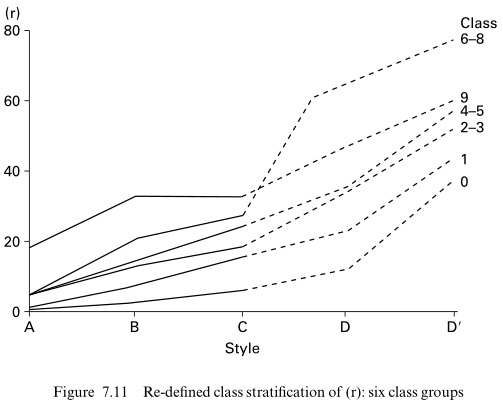
\includegraphics[scale=0.375]{hypercorrection.jpg}
          \end{columns}
        }
        \only<4>{
          \begin{block}{Standard varieties by country}
            \begin{itemize}
              \item US $\rightarrow$ Standard American English (SAE)
              \item UK $\rightarrow$ Received Pronunciation (RP)
            \end{itemize}
          \end{block}
        }
      \end{frame}

      \begin{frame}{\subtwosix}
        \begin{block}{Non-standard varieties are just as systematic}
          \parbox{0.48\linewidth}{
            \begin{tabular}{l l}
              Standard               & Non-standard \\
              \hline
              myself                 & myself \\
              yourself               & yourself \\
              \alert<2->{him}self    & hisself \\
              herself                & herself \\
              ourselves              & ourselves \\
              yourselves             & yourselves \\
              \alert<2->{them}selves & theirselves
            \end{tabular}
          }
          \parbox{0.48\linewidth}{
            \uncover<2->{
              \lexi{Him} and \lexi{them} are not chosen in the same way as the others
            }
          }
        \end{block}
      \end{frame}

      \begin{frame}{\subtwosix}
        \begin{block}{Why do non-standard varieties persist?}
          \uncover<2->{
            \alert{Covert prestige} \parencite{labov_social_2006}: % Covert prestige
The prestige carried by non-standard varieties due to how their use helps one to be favorably regarded by and identified with one's peers

          }
        \end{block}
      \end{frame}

    \subsection{\subtwoseven}
      \begin{frame}{\subtwoseven}
        \begin{block}{Try these}
          \textcite{dawson_language_2016}, chapter 10 exercise 10
        \end{block}
      \end{frame}

      \begin{frame}{References}
        \printbibliography
      \end{frame}
\end{document}
